\documentclass[a4paper,chapter,atbegshi]{oblivoir}
\usepackage[dbl4x6]{fapapersize}
\usepackage{amsmath,amssymb,amsfonts}
\usepackage{graphicx,xcolor,caption}
\usepackage{braket,hyperref,nicematrix}
\hypersetup{
colorlinks=true,linkcolor=teal,filecolor=magenta,urlcolor=cyan,
}
\newcommand{\comb}[2]{{}_{#1}\mathrm{C}_{#2}}

\title{양자정보학 학습 일지}
\author{김태원}
\date{최초 작성 : 2023년 8월 21일 \\ 최근 편집 : \today}

\begin{document}
\maketitle

\chapter{정보와 물리학}
대다수 물리학자가 프로그래밍을 따로 배우지 않고 거의 모든 전산학자가 양자역학에
관심도 없을 텐데 `양자정보학'이라니! 애초에 정보가 물리적이며 정보를 물리학으로
다룰 수 있다는 증거라도 있는가? 

있다. 바로 \emph{란다우어의 원리\tiny Landauer's principle}다.
1961년 IBM의 연구원 란다우어{\tiny Rolf Landauer}가 내놓았으며 정보 소실과
엔트로피의 관계를 나타내는 원리다. 여기서 엔트로피는 열역학의 개념으로, 
무려 열역학 제2법칙에 관한 개념이니 중요할 것이 분명하다. 열역학 제2법칙은
외부와 상호작용하지 않는 계{\tiny system}인 고립계{\tiny isolated system}의
엔트로피가 절대 감소하지 않는다고 말한다. 그런데 엔트로피가 무엇인가? 

1824년 프랑스에 가보자. 물리학자 카르노{\tiny Sadi Carnot}는 군사학자이기도
해서 열기관을 실험할 기회가 많았는데, 열이 고온에서 저온으로 떨어져서 원동력이
발생한다는 결과를 책으로 남긴다.

1862년 독일에서 이 결과를 접한 물리학자 클라우지우스{\tiny Rudolf Clausius}는 
열이 고온에서 저온으로 떨어져서 원동력이 발생한다는 결과에는 동의했지만, 
원동력의 대상에 변함이 없다는 가정에는 동의하지 않았다. 다시 말해 어떤
대상의 열이 고온에서 저온으로 떨어져 원동력이 발생할 때, 대상은 반드시
변한다. 클라우지우스는 그 변화를 변환내용{\tiny Verwandlungsinhalt}이라고
불렀고, 이는 순간의 온도 $T$와 열의 극미한 변화량 $\textrm{d}Q$에 대해 
아래 같은 양 $S$다.
\begin{equation}
  \textrm{d}S = \frac{\textrm{d}Q}{T}
\end{equation}
클라우지우스는 1865년 $S$를 (`에너지'의 `en'과 그리스어로 `변환'을 뜻하는
`트로페'{\tiny τροπή}를 따서) \emph{엔트로피\tiny entropy}라고 불렀다. 그런데
위의 경우처럼 대상에 미친 변화의 양 $dS$가 주어진 온도에 대한 열의 변화량과
일치한다면, 그만큼 차갑게 해서 대상을 원래대로 되돌릴 수 있을 것이다. 여기서
원래대로 되돌릴 수 있다는 말을 \emph{가역\tiny reversible}이라고 한다. 대상에
미친 변화의 양이 주어진 온도에 대한 열의 변화량보다 크다면, 즉 아래의 경우
\begin{equation}\label{eq:12}
  \textrm{d}S > \frac{\textrm{d}Q}{T}
\end{equation}
아무리 정확하게 차갑게 하더라도 대상을 원래대로 되돌릴 수는 없을 것이다. 여기서
되돌릴 수 없다는 말을 \emph{비가역}이라고 한다. 아무튼 핵심은 대상에 미친 변화
혹은 엔트로피 $S$의 변화량이 주어진 온도에 대한 열의 변화량보다 적을 수는 없다는
사실이다. 고립계의 엔트로피는 감소하지 않는다는 것, 이게 바로 열역학 제2법칙이다.

그런데 그래서 대상에 미친 변화, 엔트로피 자체는 무엇인가? 오스트리아의
볼츠만{\tiny Ludwig Boltzmann}은 확률이라는 풀이를 꺼낸다. 계에는 여러
미시상태{\tiny micro states}가 있을 수 있는데, 이를테면 세 동전(의 계)에 대해
앞과 뒤로 지닐 수 있는 상태는 아래와 같다.
\begin{align*}
  &\footnotesize[\comb{n}{r}\textrm{은 $n$개에서 $r$개를 선택하는 경우의 수}]\\
  &\textrm{앞}\times3 \longrightarrow \comb{3}{3}=1\\ 
  &\textrm{앞}\times2\longrightarrow\comb{3}{2}=3\\
  &\textrm{앞}\times1\longrightarrow\comb{3}{1}=3\\
  &\textrm{앞}\times0\longrightarrow\comb{3}{0}=1\\
  &\textrm{거시상태}=4,\textrm{미시상태}=1+3+3+1=8
\end{align*}
즉 미시상태는 계가 지닐 수 있는 상태의 확률을 나타내고, 다시 이를 나타내는 것이
엔트로피 $S$다. 그리하여 $\Omega$가 계에 대한 미시상태의 개수라고 할 때,
엔트로피 $S$는 $\Omega$의 자연로그 $\ln\Omega$에 비례하는 수다. 즉 아래와 같다.
\begin{equation}\label{eq:13}
  S=k_B\ln\Omega
\end{equation}
여기서 비례를 나타내는 상수 $k_B$는 ``볼츠만이 $\cdots$ 엔트로피와 확률론 
간의 로그적인 연관을 최초로 주장했다''고 요약한 플랑크{\tiny Max Planck}의
작품이다. 그리고 이 볼츠만-플랑크 엔트로피 정의가 엔트로피라는 개념을 
통상 ``무질서도''라는 일상어로 설명할 수 있는 근거다. 이를테면 구름은 
얼음보다 무질서도, 곧 엔트로피가 더 높은데, 왜냐하면 구름 속 물 분자들이
취할 수 있는 미시상태의 개수가 얼음의 구조가 허락하는 것보다 많기 때문이다. 

이에 폰 노이만{\tiny John von Neumann}이 1927년 행렬과 연산자로 볼츠만-플랑크 
엔트로피 개념을 양자역학의 계에 번역했고, 1948년 섀넌{\tiny Claude Shannon}은
미시적인 물리계가 아니라 거시적인 디지털계에 볼츠만의 엔트로피 개념을 사용하여
정보이론을 창시한다. 이때 엔트로피의 단위로 쓰인 볼츠만 상수 $k_B$는 \emph{비트}가
된다. 

그러나 이후 양자역학과 정보이론은 딱히 친하게 지내지 않았다. 물리학자는
정보나 계산을 얘기할 필요도 권리도 없었고, 정보-전산학자는 열역학이나 양자역학을
얘기할 필요도 권리도 없었다. 이에 란다우어의 원리는 정보가 물리(학)적이라고
공표한다. 

란다우어의 원리에 따르면 한 비트의 정보는 마법처럼 사라지지 않는다.
한 비트의 정보를 제거할 때는 어떤 에너지가 열로 소모되며, 그 에너지 $E$는 적어도
아래와 같다. 
\begin{equation}
  E\geq k_B T \ln 2
\end{equation}
보시다시피 볼츠만-플랑크의 엔트로피 공식 \ref{eq:13}과 아주 비슷하게 생겼다.
즉 한 비트(라는 계이자 정보의 단위)를 제거할 때 외부로 빠져 나가는 열에너지
$E$는 미시상태의 개수 $\Omega$가 $2$인 비트에 대한 엔트로피보다 크거나 같다는
것이 란다우어의 원리다.

그런데 왜 같은 것도 아니고 크거나 같아야 하는가? 엔트로피의 변화량이 주어진 온도에
대한 열의 변화량보다 큰 경우를 나타낸 공식 \ref{eq:12} ($\textrm{d}S>
\textrm{d}Q/T$)상의 부등호가 비가역성을 가리킨다는 사실을 힌트로 삼으면,
란다우어의 원리가 \emph{비가역적 계산\tiny reversible computation}에 대해 
적용된다고 유추할 수 있겠다. 가령 컴퓨터 및 전자공학도라면 익숙할 NAND 게이트가
있다고 하자. 
\[
  (a,b) \rightarrow \neg(a \wedge b)
\]
두 비트가 입력되고 하나의 비트만 출력되기에 출력 비트로 입력 비트를 복구하는
것은 불가능하다. 비가역적인 셈이다. 또한 입출력 과정에서 하나의 비트가 제거되므로,
란다우어의 원리에 의해 NAND 게이트의 연산에는 적어도 $W=k_BT\ln2$ 만큼의 열이
발생한다. 따라서 수행할 수 있는 계산에는 (컴퓨터가 녹아내린다는) 이론(물리학)적인
한계가 존재한다. 

그러나 1973년 베넷{\tiny Charles Bennett}\footnote{재밌는 사실: 찰스 베넷은 2011년
부경대에 방문했다. \url{https://www.etnews.com/201108210026}}이 
모든 (비가역) 계산을 가역 게이트로 구성할 수 있다는 사실을 보였다. 
실제로 NAND 게이트를 가역으로 구성할 수도 있다. 토폴리{\tiny Toffoli} 게이트를
사용하면 된다. 
\[
  (a,b,c)\rightarrow(a,b,c\oplus a \wedge b)
\]
첫 두 비트가 $1$이면 세 번째 비트를 뒤집고, 그게 아니라면 아무것도
하지 않는 $3$비트 게이트다. 곰곰이 생각하면 NAND와 똑같이 기능하지만 가역이라는
사실을 확인할 수 있다. 그런데 이처럼 모든 (비가역적) 계산을 가역적인 절차로
수행할 수 있다면, 란다우어의 원리의 쓸모란 무엇인가? 

그러자 어디선가 (말 그대로) 악마 하나가 모습을 드러낸다. 이른바 
\emph{멕스웰의 악마}, 1871년 맥스웰{\tiny James Maxwell}이 고안한 사고 실험이다. 

한 상자 속에 기체의 혼합물이 있고, 이 상자에는 $A$와 $B$라는 공간이 있다.
$A$와 $B$는 악마가 열고 닫을 수 있는 문으로 나뉜다. 악마는 두 종류의 기체 분자를
양쪽 공간으로 분리하고자 한다. 악마는 (악마니까 엄청 빨라서) 분자를 하나씩 관찰할
수 있다. 따라서 악마는 문을 조금씩 열고 닫으면서 빠른 분자는 $B$에 몰아넣고 느린
분자는 $A$에 몰아넣는다. 그리하여 상자는 느린 분자의 공간 $A$와 빠른 분자의 공간
$B$로 완벽하게 분리된다. 문제는 악마가 (악마니까 엄청 빨라서) 아무 분자도
건드리지 않은 채 문을 열고 닫았다는 사실이다. 즉 상자는 고립계, 악마와 기체
혼합물이 전혀 상호작용하지 않는 계다. 그런데도 방의 엔트로피가 감소했다.
고립계의 엔트로피는 감소하지 않는다는 열역학 제2법칙이 악마에게 굴복한 꼴이다. 

1982년 베넷은 란다우어의 원리로 악마를 퇴마하고자 했다. 악마가 분자의
\emph{정보를 관측}한다는 사실에 주목하면 된다. 그런데도 앞서 언급한 것처럼 모든
계산은 가역적인 절차로 변환할 수 있으며 관측 또한 계산의 일종이다. 그러니 
이것만으로는 란다우어의 원리에 의해, 즉 비가역적 계산에 대해 비트의 엔트로피보다
크거나 같은 열에너지가 발생하므로 사실 엔트로피는 증가했다고 \emph{말할 수 없다}.

그런데도 란다우어의 원리가 한 발 남았다. 우선 악마 또한 뇌와 같은 기억 공간을
지니기에, 메모리상 제약을 지닌다는 사실에 주목하겠다. 메모리가 다 차서
더는 (가역이든 비가역이든) 계산을 수행할 수 없으면 악마는 어떻게 할 것인가?
\emph{메모리에서 쓸데없는 정보를 지워야 할 것}이다. 정보 제거라는 정보처리를
향해 란다우어의 원리를 쏘면, 한 비트의 정보를 제거할 때 열에너지가 발생한다는
사실에 의해, 엔트로피는 증가한다. 고립계의 엔트로피가 감소하지 않았으므로
열역학 제2법칙을 지켜냈고, 악마를 물리쳤다. 

컴퓨터도 나날이 작아지는데, 란다우어의 원리를 분명하게 고려하지 않으면 화재나
폭발이 발생하리라는 게 교훈이다. 아무튼 이렇듯 물리학의 개념적인 문제를
해결하기 위해 정보 혹은 계산의 개념이 요구된다. 역으로 정보 혹은 계산, 다시 말해
전산학의 문제를 해결하기 위해 물리학, 정확히 말해 양자역학의 개념이 요구되기도
한다. 

\emph{처치-튜링 논제}를 보자. 처치-튜링 논제에 따르면 계산 가능한 함수는 모두
튜링장치로 계산할 수 있다. 즉 모든 컴퓨터는 근본적으로 똑같다. 전산학의
기저를 이루는 근본 (정리가 아니라) 믿음이다. 문제는 \emph{확장 처치-튜링 논제}라는
것이다. 이에 따르면 \emph{효율적으로} 계산 가능한 함수는 모두 튜링장치에 의해
\emph{효율적으로} 계산할 수 있다. 

이 또한 믿음으로, 악마까지는 아니라도 불쾌한 것이라고들 한다. 그런데 양자역학,
정확히 말해 양자정보학은 확장 처치-튜링 논제를 박살낸다. 이 광경을 충분히 묘사할
수 있는 능력을 지니는 것이 양자정보학 학습의 목적 가운데 하나다. 최우선으로 필요한
도구는 \emph{새로운 확률론}이다. 

\chapter{새로운 확률론 (작성 중)} 
우리는 이미 확률을 알고 있다. 동전을 던졌을 때 위가 나올 확률과 밑이 나올 확률은
각각 $0$ 이상이며 합하면 $1$이다. 대단히 자연스럽다. 그런데 (양자역학적) 자연은
이렇게 굴러가지 않는다. 이와 같은 고전 확률론에 따라 던진 동전이라는 계의 일종은
제 환경과 상호작용한다. 그리고 인간은 계와 상호작용을 직관적으로 분리할 수 없다.
이를 \emph{결어긋남\tiny decoherence}이라고 부른다.

비슷하게 그 유명한 슈뢰딩거의 고양이가 생과 사라는 상태의 중첩{\tiny
superposition}으로 발견되지 않는 이유는 바로 결어긋남으로, 고양이가 끊임없이
제 환경과 상호작용하기 때문이다. 양자 중첩은 입자를 제 환경과 격리{\tiny
isolate}할 때 일어나는 일이다. 그리고 이게 양자컴퓨터를 만들기 어려운 이유다.

(필자는 고등학교를 다니지 않아서 모르겠지만) 고교 과학 시간에 나오는 것처럼
핵을 중심으로 회전하는 전자가 있다고 하자. 20세기 초 과학자들은 전자가 에너지를
상실하며 핵과 충돌할 때까지 나선 운동을 한다고 봤다. 문제는 전자의 궤도가
안정적이라는 사실이다. 그리고 이런 안정성과 이중 슬릿 실험을 비롯한 결과들을
설명하기 적합한 도구는 고전적인 확률론이 아니라 \emph{진폭\tiny amplitude}이었다.

앞서 언급한 것처럼 고전적인 확률은 $P\in[0,1]$, 다시 말해 $101\%$나 $-1\%$ 같은
확률이 존재할 수는 없다. 그런데 진폭 $\alpha$는 복소수다. 또 \emph{보른 규칙}에
따르면 특정 결과를 보는 확률은 진폭의 절댓값을 제곱한 것과 같다. 보른 규칙은
양자역학의 핵심 가정으로, 보른{\tiny Max Born}이 1926년 슈뢰딩거 방정식의
파동함수를 해석하는 가운데 내놓았다. 보른 규칙이 핵심적인 이유는 이 규칙이
실험 결과와 딱 들어맞는 `해석'이기 때문이다. 여기에 엄청난 세계관이 담긴 것은
아니고 아무튼 정말 딱 들어맞기 때문이다. (이를 `코펜하겐 해석'이라고 부른다)
\begin{equation}\label{eq:11}
P=|\alpha|^2
\end{equation}
보른 규칙 \ref{eq:11}을 사용해 이중 슬릿 실험을 전개해 보자. 우선 $\alpha$를 
광자가 스크린상의 특정 지점에 부딪히는 총 진폭이라고 하자. 그리고 $\alpha_1$은
1번 슬릿만 열린 경우 부딪히는 진폭, $\alpha_2$는 2번 슬릿만 열린 경우 부딪히는
진폭이라고 하자. 보른 규칙 \ref{eq:11}에 따르면 두 슬릿 모두 열린 경우
광자가 특정 지점에 부딪히는 확률 $P$는 아래와 같다.
\begin{align*}
  P &= |\alpha|^2 \\ 
    &= |\alpha_1+\alpha_2|^2 \\ 
    &= |\alpha_1|^2 + |\alpha_2|^2 + \overline{\alpha_1}\alpha_2+\alpha_1\overline{\alpha_2}
\end{align*}
$\alpha_1=\frac{1}{2},\alpha_2=-\frac{1}{2}$의 진폭으로 두 슬릿이 모두 열리면
$P=0$이지만 둘 중 하나의 슬릿만 열리면 $P=\frac{1}{4}$로, 경우의 수를 늘리니까
오히려 확률이 줄어든 셈이다. 이중 슬릿 실험과 딱 맞는 결과이며, 이는 전자의 
나선 궤도가 안정적인 이유와 같다. 어떤 경로는 양의 진폭을 지니고 어떤 경로는
음의 진폭을 지녀 서로 소거하는 것이다. 이런 현상을 \emph{간섭\tiny
interference}이라고 부른다.  

진폭을 다루려면 복소행렬 혹은 어떤 특별한 변환들이 필요하다. 가령 아래 $4\times 4$
행렬은 통제된 NOT 혹은 CNOT이라고 부르는 변환이다. 
\begin{equation}
  \textrm{CNOT } = 
  \begin{bNiceMatrix}[first-col, first-row]
    & \scriptstyle00 & \scriptstyle01 & \scriptstyle10 & \scriptstyle11 \\
    \scriptstyle00 & 1 & 0 & 0 & 0 \\
    \scriptstyle01 & 0 & 1 & 0 & 0 \\
    \scriptstyle10 & 0 & 0 & 0 & 1 \\
    \scriptstyle11 & 0 & 0 & 1 & 0
  \end{bNiceMatrix}
  \label{eq:212}
\end{equation}
첫 비트가 $0$이면 두 번째 비트를 그대로 두고, 첫 비트가 $0$이 아니면 두 번째
비트에 $2$를 법으로 하여{\tiny mod 2} $1$을 더하는 변환이다. 이 변환을
$\frac{1}{2}$의 확률로 첫 비트가 $0$이거나 $1$이며 두 번째 비트는 항상 $0$인
계에 적용한 분포는 아래와 같다.
\begin{equation}
  \begin{bmatrix}
    1&0&0&0\\0&1&0&0\\0&0&0&1\\0&0&1&0
  \end{bmatrix}
  \begin{bmatrix}
    \frac{1}{2}\\0\\\frac{1}{2}\\0
  \end{bmatrix}
  =
  \begin{bNiceMatrix}[first-col]
    {\scriptstyle 00} & \frac{1}{2} \\
    {\scriptstyle 01} & 0 \\
    {\scriptstyle 10} & 0 \\
    {\scriptstyle 11} & \frac{1}{2}
  \end{bNiceMatrix}
\end{equation}
이 분포는 텐서곱으로 구성될 수 없다. 다시 말해 아래 같은 연산은 있을 수 없다.
\begin{equation}
  \begin{bmatrix}ac\\ad\\bc\\bd\end{bmatrix}
  =\begin{bmatrix}\frac{1}{2}\\0\\0\\\frac{1}{2}\end{bmatrix}\quad\quad
\begin{aligned}
   (ac)(bd) &= \frac{1}{4} \\
  \Leftrightarrow  (ad)(bc) &= \frac{1}{4} \\
              &\neq 0\rightarrow\textrm{ 모순}
\end{aligned}
\end{equation}
이처럼 한 비트에 관한 정보가 두 번째 비트에 관한 정보를 제공하는 분포를
\emph{상호연관되어 있다\tiny correlated}고 한다. 핵심은 CNOT 행렬이 
상호연관을 만들어냈다는 사실이다. 물론 위 사례 속 분포는 실수, 즉 고전적인
확률에 따른 것이니, 여기서 보른 규칙 \ref{eq:11}에 따라 확률의 개념만 
진폭으로 바꾸면 된다. 
\begin{equation}\label{eq:15}
  \sum_{i=1}^3 |a_i|^2 = 1 = \sum_{i=1}^3 |b_i|^2\textrm{를 만족하는 $a_i,b_i$에 대해 }
  \begin{bmatrix}
    & & \\ & U & \\ & &
    \end{bmatrix}\begin{bmatrix}a_1\\a_2\\a_3\end{bmatrix}
    =\begin{bmatrix}b_1\\b_2\\b_3\end{bmatrix}
\end{equation}
이처럼 보른 규칙을 보존하는 행렬 $U$ \emph{유니터리 행렬\tiny unitary
matrix}이라고 부른다. 이건 뭔가? 새로운 확률론과 더불어 행렬 혹은 벡터의 
새로운 표기법을 취할 차례다. 이로써 사실상 양자정보를 소화할 수준의
양자역학 기초를 취할 수 있다. 

\chapter{양자역학 기초}
줄곧 상태{\tiny state}라는 말을 사용했는데, 양자계의 경우 상태란 
$\mathbb{C}^N$상의 단위 벡터를 뜻한다. 필자는 물리학도가 아니기 때문에 $N$이
유한하다고 가정하겠다. 우선 \emph{큐빗\tiny qubit}이라는 아주 간단한
양자계로 시작하겠다. 큐빗은 $0$에 대한 진폭과 $1$에 대한 진폭을 지닌다. 또한
\emph{켓\tiny ket} 표기를 도입한다.
\[
  \ket{0}=\begin{bmatrix}1\\0\end{bmatrix},\ket{1}=\begin{bmatrix}0\\1\end{bmatrix} 
  \Rightarrow\begin{bmatrix}\alpha\\\beta\end{bmatrix}=
  \alpha\ket{0}+\beta\ket{1}=\ket{\psi}
\]
벡터공간 $\mathbb{C}^N$상의 벡터 $\psi$의 노름 혹은 크기는 $\psi$의 전치켤레에 $\psi$를
곱한 것이다.
\[
  \|\psi\|^2 = \begin{bmatrix}\overline{\alpha}&\overline{\beta}\end{bmatrix}
  \begin{bmatrix}\alpha\\\beta\end{bmatrix} = |\alpha|^2 = |\alpha|^2 + |\beta|^2
\]
또한 \emph{브라\tiny bra} 표기를 도입한다. (합쳐서 브라-켓이다)
\[
  \bra{\psi} = \overline{\alpha}\bra{0}+\overline{\beta}\bra{1}
  =\begin{bmatrix}\overline{\alpha}&\overline{\beta}\end{bmatrix}
\]
노름의 정의를 돌아보면 내적을 그냥 아래처럼 표현할 수 있겠다.
\[
  \braket{x|y}=\overline{\braket{y|x}}
\]
표준 단위 기저 혹은 표준 단위 양자 상태는 $\ket{0},\ket{1}$이겠다. 
좀 더 특이하고 (나중에 이름도 수여할 만큼) 대단히 중요한 단위 벡터로는 아래
같은 것들이 있다.
\[
  \ket{+}=\frac{\ket0+\ket1}{\sqrt{2}}, \ket{-}=\frac{\ket{0}-\ket{1}}{\sqrt{2}},
  \ket{i}=\frac{\ket0+i\ket1}{\sqrt{2}}, \ket{-i}=\frac{\ket0-i\ket1}{\sqrt2}
\]
방정식 \ref{eq:15}에서 처음 언급한 $U$라는 행렬로 선형 변환을 사용해 양자계의
상태를 바꾸는 법을 보자.
\[
  U\ket{\psi} = U\begin{bmatrix}\alpha\\\beta\end{bmatrix}
  =\begin{bmatrix}\alpha'\\\beta'\end{bmatrix}
\]
단일 큐빗에 대한 변환 $U$가 유니터리라는 말은 모든 입력 벡터 $\begin{bmatrix}
\alpha\\\beta\end{bmatrix}$에 대해 아래를 만족한다는 뜻이다.
\[
  |\alpha|^2+|\beta|^2 = |\alpha'|^2+|\beta'|^2
\]
다시 말해 유니터리 행렬 $U$는 벡터의 노름을 보존하고, 내적의 값도 보존한다.
아래는 유니터리 변환의 예다.
\begin{align*}
  \textrm{항등 변환: }& \begin{bmatrix}1&0\\0&1\end{bmatrix} \\
  \textrm{NOT 게이트: }&\begin{bmatrix}0&1\\1&0\end{bmatrix}\\
  \textrm{2D 회전: }&\begin{bmatrix}\cos\theta &-\sin\theta\\\sin\theta &\cos\theta\end{bmatrix}
\end{align*}
눈치 챘겠지만 유니터리 행렬의 전치행렬 $U^{\dagger}$는 $U$의 역행렬이다.
\begin{equation}
  \braket{\psi|\psi}=(\ket{\psi})^{\dagger}\ket{\psi}=(U\ket{\psi})^{\dagger}U\ket{\psi}=\braket{\psi|U^{\dagger}U|\psi} \iff U^{\dagger}U= I
\end{equation}
앞서 언급한 간섭 또한 유니터리 변환으로 설명할 수 있다. $\ket0,\ket1$에
대해 각각 $\ket+=\frac{\ket0+\ket1}{\sqrt2},\ket-=\frac{\ket0-\ket1}{\sqrt2}$를
내놓는 변환을 반복한다고 하자. 각 경로에 대해 트리가 만들어질 것이다. 아래는
초기값을 $\ket0$으로 뒀을 때의 트리다.

\begin{center}
  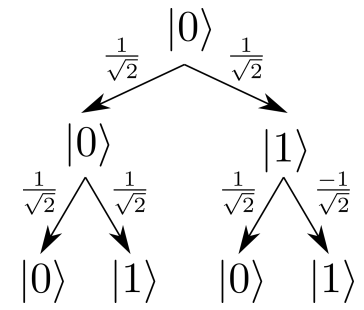
\includegraphics[width=0.3\textwidth]{qis001}
\end{center}

특정 경로의 진폭을 취하려면 그 경로를 따라 진폭의
곱을 취해야 한다. 특정 출력에 대한 마지막 진폭을 취하려면, 출력으로 이어지는
트리를 따르는 각 경로에 대해 진폭을 합해야 한다. 이 경우, $\ket0$의 진폭은 
$1$이고 $\ket1$의 진폭은 $0$이다. $\ket0$에 이르는 경로는 구성적으로 간섭하고,
$\ket1$에 이르는 경로는 파괴적으로 간섭한다.

\end{document}
